\documentclass[hyperref={unicode}]{beamer}
%
% Choose how your presentation looks.
%
% For more themes, color themes and font themes, see:
% http://deic.uab.es/~iblanes/beamer_gallery/index_by_theme.html
%
\mode<presentation>
{
  \usetheme{Antibes}      % or try Darmstadt, Madrid, Warsaw, ...
  \usecolortheme{dolphin} % or try albatross, beaver, crane, ...
  \usefonttheme{professionalfonts}  % or try serif, structurebold, ...
  \setbeamertemplate{navigation symbols}{}
  \setbeamertemplate{caption}[numbered]
  % Numbered bibiolgraphy items
  \setbeamertemplate{bibliography item}{\insertbiblabel}
}

\usepackage[utf8]{inputenc}
\usepackage[english]{babel}
\usepackage[T1]{fontenc}
\usepackage{csquotes,lmodern,silence,multicol}
\usepackage[style=numeric-comp,backend=biber]{biblatex}

\WarningFilter{biblatex}{Patching footnotes failed}

% Remove small caps warning
\renewcommand\mkbibacro[1]{{\footnotesize\MakeUppercase{#1}}}

\addbibresource{fuzzy_logic.bib}
\graphicspath{{figures/}}

\title[Fuzzy logic]{Fuzzy Logic}
\author{Peter Babič}
\institute{Technical University of Košice, Slovakia}
\date{18.05.2015}

\begin{document}
\boldmath


\begin{frame}
	\titlepage
\end{frame}

\begin{frame}{Presentation Outline}
%\begin{multicols}{2}
  \tableofcontents
%\end{multicols}
\end{frame}



\section{Introduction}


\subsection{Crisp and Fuzzy Logic}

\begin{frame}{Introduction to Fuzzy logic}
	\begin{columns}
	\column{.6\textwidth}
		\begin{itemize}
		\item Fuzzy logic is an extension of multivalued logic
		\item Natural language rules
		\item Aristotle, later Lofti A. Zadeh in 1965 and 1973
		\item Japan, later on west
		\end{itemize}

	\column{.35\textwidth}
		\begin{figure}[b]
		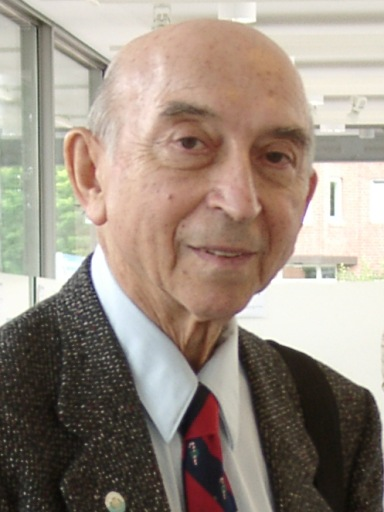
\includegraphics{lofti}
		\caption{Lofti A. Zadeh}
		\end{figure}
	\end{columns}
\end{frame}


\begin{frame}{Fuzzy logic vs Crisp logic}
	\begin{exampleblock}{Example}
	Carmen is 18 years old. Is she old?
	\end{exampleblock}

	\begin{itemize}
		\setlength{\itemindent}{2cm}
		\item[Crisp\footnote{In this context referred also as a \emph{Boolean} or \emph{bivalent} logic}] \textbf{true}/\textbf{false}
		\item[Fuzzy]  \textbf{true}, \textbf{false} or the \textbf{degree} of \textit{oldness}
	\end{itemize}

	\begin{figure}
	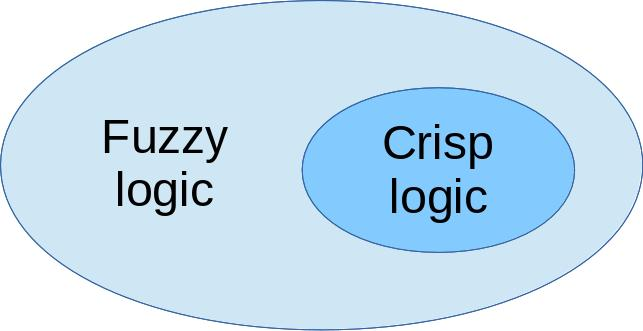
\includegraphics[width=.5\textwidth]{fuzzy-crisp}
	\caption{The classical set theory is a subset of the theory of fuzzy sets}
	\end{figure}
\end{frame}

\begin{frame}{Crisp Set}
	Theory of Sets (formerly Classes) was conceptualized by George Cantor in 1870's.
	\begin{figure}
	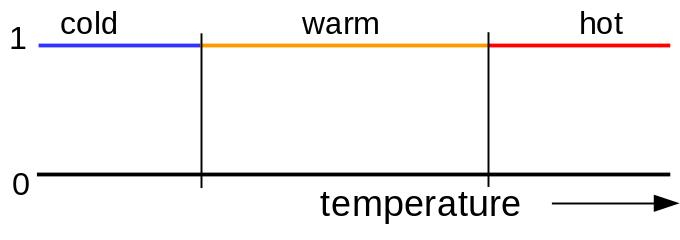
\includegraphics[width=.75\textwidth]{crisp-set}
	\caption{Crisp set illustration. The element either is fully member of a set or is not a member at all.}
	\end{figure}
\end{frame}

\begin{frame}{Sorites Paradox}
	When does a heap of grains stops being heap, if we are removing one grain at a time?

	\begin{figure}
	
\includegraphics[width=.75\textwidth]{sorites-gradient}
	\caption{At what point exactly does blue becomes red? Sorites paradox \cite{podosky1985vagueness}.}
	\end{figure}

	$$Bald(0)$$
	$$Bald(n)\rightarrow Bald(n+1)$$
	$$\therefore Bald(10000)$$
\end{frame}

\subsection{Fuzzy Sets}

\begin{frame}{Fuzzy Sets}
	In mathematics, fuzzy sets are sets whose elements have \textit{degrees} of membership, described by a \textit{membership function} \cite{buckley2002introduction}.

	\vskip .5cm
	\begin{itemize}
		\item Degree of membership is defined in interval\footnote{In theory, it could be higher than 1, but in practice it is almost never used} $[0, 1]$
		\item Elements can have different degree of membership to different fuzzy sets
		\item If the uncertainty is not handled, we talk about \textbf{type-1} fuzzy sets, \textbf{type-2} otherwise
	\end{itemize}
\end{frame}

\begin{frame}{Fuzzy Set Interpretation}
	How do we represent \textit{numerical} value in a fuzzy set? With the use of \textit{linguistic variables} \cite{lieb1993linguistic}, \textbf{not} probabilities.
	\begin{figure}
		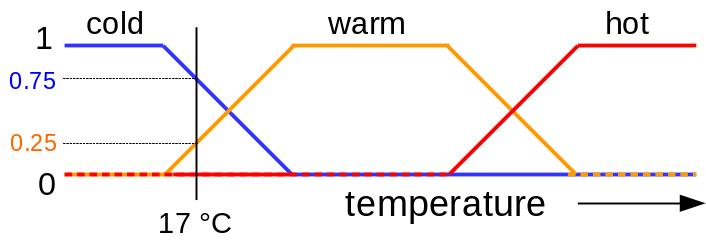
\includegraphics[width=.75\textwidth]{fuzzy-set-degrees}
		\caption{Example interpretation of fuzzy sets. At the given temperature point, we can tell that the measured medium is "not hot", "slightly warm" and "almost cold". It does not mean that the chance the water is cold is 75\%.
		\label{fig:fuzzy-set}}
	\end{figure}
\end{frame}

\begin{frame}{Formal Definitions}
	\begin{block}{Definition}
		Let $U$ be the \textit{universe of discourse} and $x$ be the element in it. The \textit{membership function} $f^A$ assigning \textit{degree of membership} $\mu_A$:
		$$f^A(x): \: \in U \rightarrow \mu_A(x) \in [0,1]$$
%		$$\mu_A:U\rightarrow[0,1]$$
	\end{block}
	\begin{block}{Definition}
		A fuzzy set $A$ is expressed as a set of ordered pairs (tuples), given that $\mu_A(x)$ is a degree, to which $x$ a member of $A$:
	$$A=\{(x,\mu_A(x))\,|\,x \in U\}$$
	\end{block}
\end{frame}

\begin{frame}{Standard Fuzzy Set Operations}
	Given that $A,B\in U$ and $u$ is an element in universe $U$:
	\vskip .5cm
	\begin{itemize}
	\setlength{\itemindent}{3cm}
	\item[Complement] $\mu_A(u)=1-\mu_A(u)$
	\item[Intersection] $\mu_{A\cap B}(u)=min\{\mu_A(u),\mu_B(u)\}$
	\item[Union] $\mu_{A\cup B}(u)=max\{\mu_A(u),\mu_B(u)\}$
	\end{itemize}

	\begin{figure}
	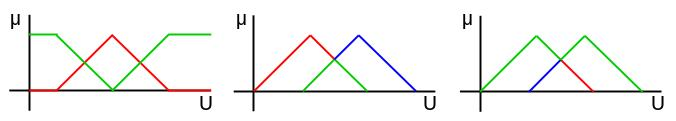
\includegraphics[width=.95\textwidth]{fuzzy-set-op}
	\caption{The complement $\mathbf{\mu_{\bar A}}$, the intersection $\mathbf{\mu_{A\cap B}}$ and the union $\mathbf{\mu_{A\cup B}}$ (green).}
	\end{figure}
\end{frame}

\begin{frame}{Fuzzy Set Operations Truth Tables}
	\begin{table}
		\caption{The truth tables for \textbf{AND}, \textbf{OR} and \textbf{NOT} operations}
		\begin{tabular}{|c|c|c|}
		\hline
		\rule[-1ex]{0pt}{2.5ex} \textbf{A} & \textbf{B} & \textbf{min(A,B)} \\
		\hline
		\rule[-1ex]{0pt}{2.5ex} 0 & 0 & 0 \\
		\hline
		\rule[-1ex]{0pt}{2.5ex} 0 & 1 & 0 \\
		\hline
		\rule[-1ex]{0pt}{2.5ex} 1 & 0 & 0 \\
		\hline
		\rule[-1ex]{0pt}{2.5ex} 1 & 1 & 1 \\
		\hline
		\end{tabular}
		\hskip .5cm
		\begin{tabular}{|c|c|c|}
		\hline
		\rule[-1ex]{0pt}{2.5ex} \textbf{A} & \textbf{B} & \textbf{max(A,B)} \\
		\hline
		\rule[-1ex]{0pt}{2.5ex} 0 & 0 & 0 \\
		\hline
		\rule[-1ex]{0pt}{2.5ex} 0 & 1 & 1 \\
		\hline
		\rule[-1ex]{0pt}{2.5ex} 1 & 0 & 1 \\
		\hline
		\rule[-1ex]{0pt}{2.5ex} 1 & 1 & 1 \\
		\hline
		\end{tabular}
		\hskip .5cm
		\begin{tabular}{|c|c|}
		\hline
		\rule[-1ex]{0pt}{2.5ex} \textbf{A} & \textbf{1-A} \\
		\hline
		\rule[-1ex]{0pt}{2.5ex} 1 & 0 \\
		\hline
		\rule[-1ex]{0pt}{2.5ex} 0 & 1 \\
		\hline
		\end{tabular}
	\end{table}

	\vskip .5cm
	It is no coincidence, that these truth tables for binary fuzzy sets are identical to their Boolean counterparts\footnote{DeMorgan's law, associativity, comutativity and distributivity also apply.}.
\end{frame}

\begin{frame}{Triangular Norm (T-norm)}
	A T-norm is a \textbf{continuous} function $T:[0,1]\times [0,1]\rightarrow [0,1]$, satisfying these axioms:
	\begin{itemize}

	\vskip .5cm
	\setlength{\itemindent}{3cm}
	\item[Neutrality\footnote{Also referred to as a \emph{boundary condition}.}] $T(a, 1) = a$
	\item[Commutativity] $T(a,b)=T(b,a)$
	\item[Monotonicity] $T(a,b) \le T(c,d)\;if\;a \le c\;and\;b \le d$
	\item[Associativity] $T(a, T(b, c)) = T(T(a, b), c)$
%	\item[Subidempotency] $T(a,a)\le a$
	\end{itemize}

	\vskip .5cm
	T-norm is used to customize the fuzzy \textbf{intersection} (conjunction).
	The fuzzy \textbf{union} (disjunction) uses the S-norm (or T-conorm).
\end{frame}

\begin{frame}{The Most Common T-norms}
	$$\mathsf{T_{min}}(a,b)=min\{a,b\}$$
	\begin{figure}
	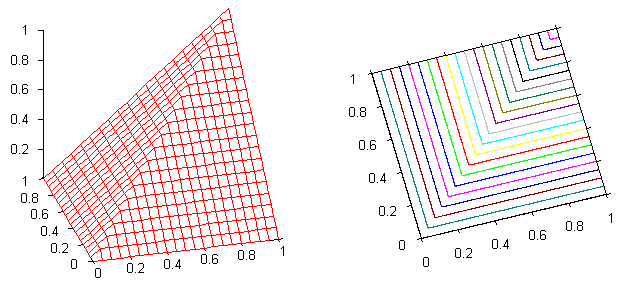
\includegraphics[width=.95\textwidth]{min-tnorm}
	\caption{\textbf{Minimum} (G{\"o}del) T-norm is the most common one}
	\end{figure}
\end{frame}

\begin{frame}{The Most Common T-norms}
	$$\mathsf{T_{prod}}(a,b)=a \cdot b$$
	\begin{figure}
	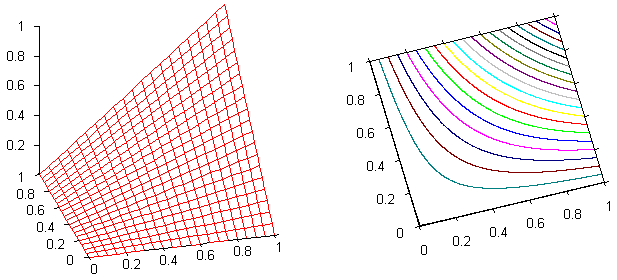
\includegraphics[width=.95\textwidth]{product-tnorm}
	\caption{\textbf{product} T-norm}
	\end{figure}
\end{frame}

\begin{frame}{The Most Common T-norms}
	$$\mathsf{T_{Luk}}(a,b)=max\{0,\:a+b-1\}$$
	\begin{figure}
	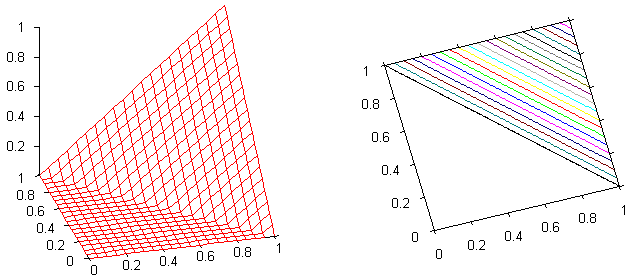
\includegraphics[width=.95\textwidth]{luk-tnorm}
	\caption{\textbf{{\L}ukasiewics} T-norm}
	\end{figure}
\end{frame}


%\addtocontents{toc}{\newpage}
\section{Applications}


\subsection{Fuzzy Control}

\begin{frame}{Fuzzy Control}
	\begin{itemize}
	\item The wider application of the fuzzy logic \cite{lughofer2011evolving}
	\item Easier to mechanize tasks that are already successfully performed by humans
	\end{itemize}

	% lughofer2011evolving, mamdani inference
	\begin{figure}
	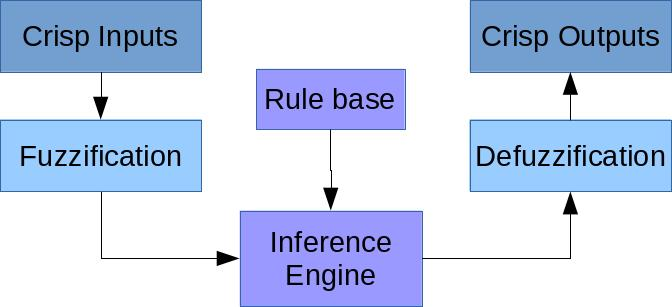
\includegraphics[width=.75\textwidth]{fuzzy-control-block}
	\caption{Block diagram of a fuzzy control}
	\end{figure}
\end{frame}

\begin{frame}{Fuzzy Inference Engine}
	\begin{figure}
	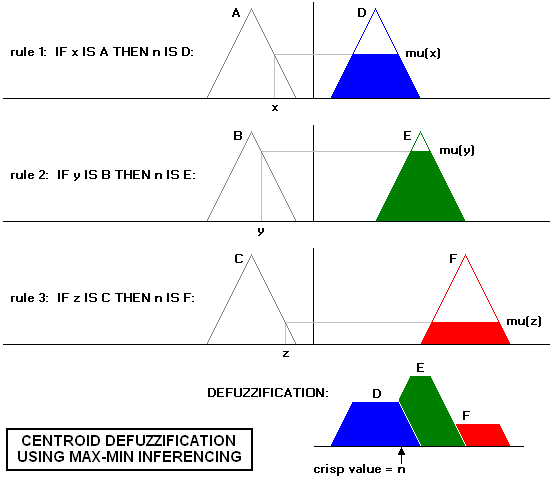
\includegraphics[width=.6\textwidth]{inference}
	\caption{Process of a fuzzy control. The most used method for defuzzification is \textit{center of gravity} (centroid).}
	\end{figure}
\end{frame}


\begin{frame}{Fuzzy Control Applications}
	\begin{itemize}
	\item Camera autofocus by Canon
	\item Increased effectivity of Mutsushita vacuum robots
	\item Mitsubishi air conditioner with higher efficiency and lower sensors
	\item Handwriting recognition, elevator systems, self-balancing robots
%	\item Simple, low cost $\rightarrow$ many more \dots
	\end{itemize}

	\vskip .5cm
	The fuzzy control systems are commonly used \cite{ross2009fuzzy} where there are not enough resources for highly advanced systems like \textbf{PID\footnote{Proportional-integral-derivative} controller}, \textbf{Artificial neural network} or \textbf{Genetic algorithm} \cite{rajasekaran2003neural}.
\end{frame}


\subsection{Software}

\begin{frame}{MATLAB Fuzzy Toolbox Introduction}
	\begin{itemize}
		\item Provides a complete set of functions to design an implement various fuzzy logic processes \cite{sivanandam2006introduction}
		\item Major fuzzy logic operation-fuzzification, defuzzification, and the fuzzy inference
		\item Can be implemented using the Graphical User Interface (GUI)
	\end{itemize}
\end{frame}

\begin{frame}{MATLAB Fuzzy Toolbox}
	 Features:
	\begin{itemize}
		\item It provides tools to create and edit fuzzy inference system (FIS).
		\item Allows integrating fuzzy systems into simulation with Simulink.
		\item It is possible to create stand-alone C programs that call on fuzzy systems
	\end{itemize}
	MATLAB Fuzzy Toolbox Tool Categories:
	\begin{itemize}
		\item Command line functions
		\item Graphical or interactive tools
		\item Simulink blocks
	\end{itemize}
\end{frame}




\begin{frame}[allowframebreaks]{MATLAB Fuzzy Toolbox}
	\begin{figure}
	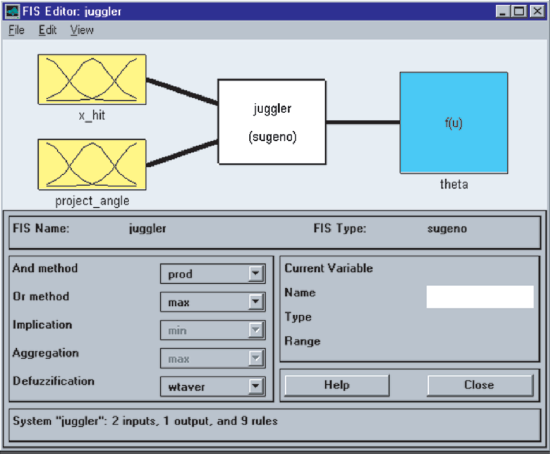
\includegraphics[width=.75\textwidth]{sw-1}
%	\caption{•}
	\end{figure}
	\begin{figure}
	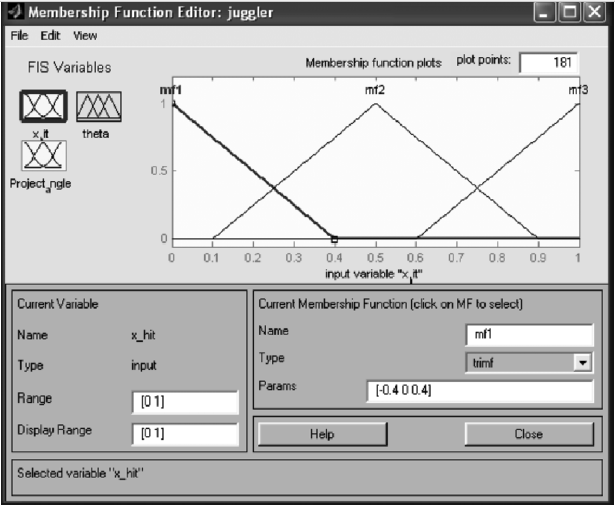
\includegraphics[width=.75\textwidth]{sw-2}
%	\caption{•}
	\end{figure}
	\begin{figure}
	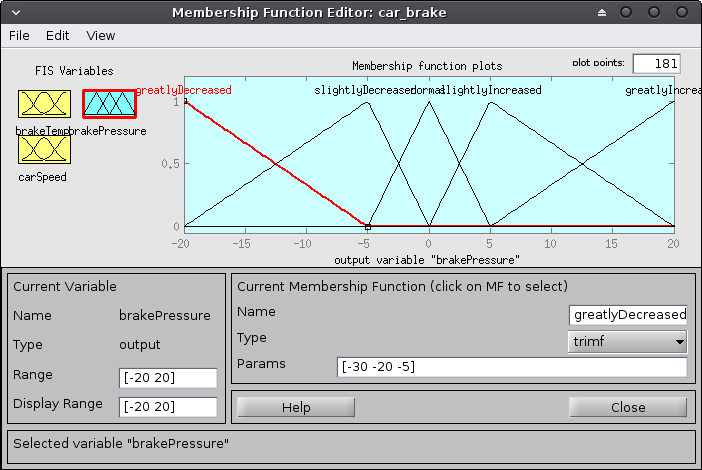
\includegraphics[width=.75\textwidth]{sw-3}
%	\caption{•}
	\end{figure}
	\begin{figure}
	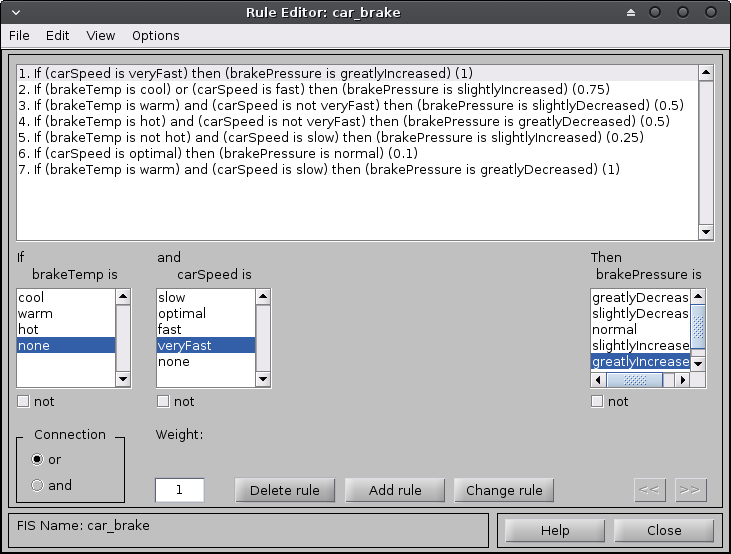
\includegraphics[width=.75\textwidth]{sw-4}
%	\caption{•}
	\end{figure}
	\begin{figure}
	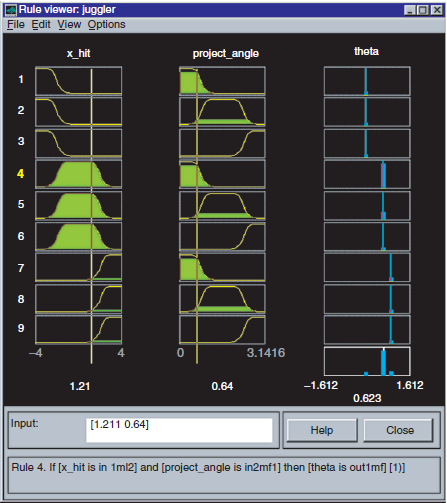
\includegraphics[width=.5\textwidth]{sw-5}
%	\caption{•}
	\end{figure}
	\begin{figure}
	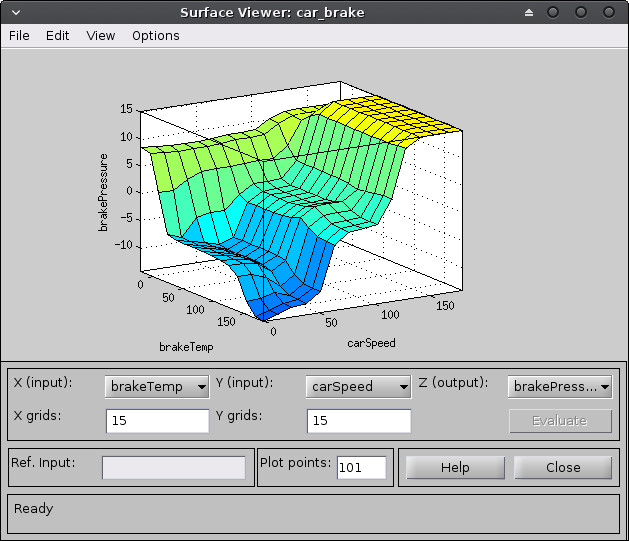
\includegraphics[width=.75\textwidth]{sw-6}
%	\caption{•}
	\end{figure}
\end{frame}


\section{Final Remarks}

\begin{frame}{Is Fuzzy Logic a Viable Option?}
	The widespread use, amount of knowledge accumulated and countless tools and literature available proof it as \textbf{yes}.
\end{frame}


\subsection{References}

\begin{frame}[allowframebreaks]{References}
	\printbibliography
\end{frame}


\subsection{Epilogue}

\begin{frame}{Questions?}
	\centering
	{\large Thank you $\cdot$ !`Gracias! $\cdot$ Ďakujem}
\end{frame}

\end{document}

%sivanandam2006introduction


%\begin{frame}{Blocks}
%
%	\begin{block}{This is a Block}
%	This is important information
%	\end{block}
%
%	\begin{alertblock}{This is an Alert block}
%	This is an important alert
%	\end{alertblock}
%
%
%	\begin{exampleblock}{This is an Example block}
%	This is an example
%	\end{exampleblock}
%
%\end{frame}


%\begin{itemize}
%\item Use \texttt{tabular} for Basic Tables! --- See Table~\ref{tab:widgets}, for Example.
%\item You Can Upload a Figure (JPEG, PNG or PDF) Using the Files Menu.
%\item to Include It in Your Document, Use the \texttt{includegraphics} Command (See the Comment Below in the Source Code).
%\end{itemize}


%\begin{table}
%\centering
%\begin{tabular}{l|r}
%Item & Quantity \\\hline
%Widgets & 42 \\
%Gadgets & 13
%\end{tabular}
%\caption{\label{tab:widgets}An example table.}
%\end{table}



%  Let $X_1, X_2, \ldots, X_n$ be a sequence of independent and identically distributed random variables with $\text{E}[X_i] = \mu$ and $\text{Var}[X_i] = \sigma^2 < \infty$, and let
%  $$S_n = \frac{X_1 + X_2 + \cdots + X_n}{n}
%  = \frac{1}{n}\sum_{i}^{n} X_i$$
%  denote their mean. Then as $n$ approaches infinity, the random variables $\sqrt{n}(S_n - \mu)$ converge in distribution to a normal $\mathcal{N}(0, \sigma^2)$.




% \vskip 1cm

% \begin{block}{Examples}
% Some examples of commonly used commands and features are included, to help you get started.
% \end{block}
